% This file is generated by the MATLAB m-file laprint.m. It can be included
% into LaTeX documents using the packages graphicx, color and psfrag.
% It is accompanied by a postscript file. A sample LaTeX file is:
%    \documentclass{article}\usepackage{graphicx,color,psfrag}
%    \begin{document}% This file is generated by the MATLAB m-file laprint.m. It can be included
% into LaTeX documents using the packages graphicx, color and psfrag.
% It is accompanied by a postscript file. A sample LaTeX file is:
%    \documentclass{article}\usepackage{graphicx,color,psfrag}
%    \begin{document}% This file is generated by the MATLAB m-file laprint.m. It can be included
% into LaTeX documents using the packages graphicx, color and psfrag.
% It is accompanied by a postscript file. A sample LaTeX file is:
%    \documentclass{article}\usepackage{graphicx,color,psfrag}
%    \begin{document}% This file is generated by the MATLAB m-file laprint.m. It can be included
% into LaTeX documents using the packages graphicx, color and psfrag.
% It is accompanied by a postscript file. A sample LaTeX file is:
%    \documentclass{article}\usepackage{graphicx,color,psfrag}
%    \begin{document}\input{interior}\end{document}
% See http://www.mathworks.de/matlabcentral/fileexchange/loadFile.do?objectId=4638
% for recent versions of laprint.m.
%
% created by:           LaPrint version 3.16 (13.9.2004)
% created on:           15-Feb-2012 20:53:18
% eps bounding box:     15 cm x 11.25 cm
% comment:              
%
\begin{psfrags}%
\psfragscanon%
%
% xticklabels:
\psfrag{x01}[t][t]{0.15}%
\psfrag{x02}[t][t]{0.155}%
\psfrag{x03}[t][t]{0.16}%
\psfrag{x04}[t][t]{0.165}%
\psfrag{x05}[t][t]{0.17}%
%
% yticklabels:
\psfrag{v01}[r][r]{1.42}%
\psfrag{v02}[r][r]{1.44}%
\psfrag{v03}[r][r]{1.46}%
\psfrag{v04}[r][r]{1.48}%
\psfrag{v05}[r][r]{1.5}%
\psfrag{v06}[r][r]{1.52}%
\psfrag{v07}[r][r]{1.54}%
\psfrag{v08}[r][r]{1.56}%
\psfrag{v09}[r][r]{1.58}%
%
% Figure:
\resizebox{0.5\columnwidth}{!}{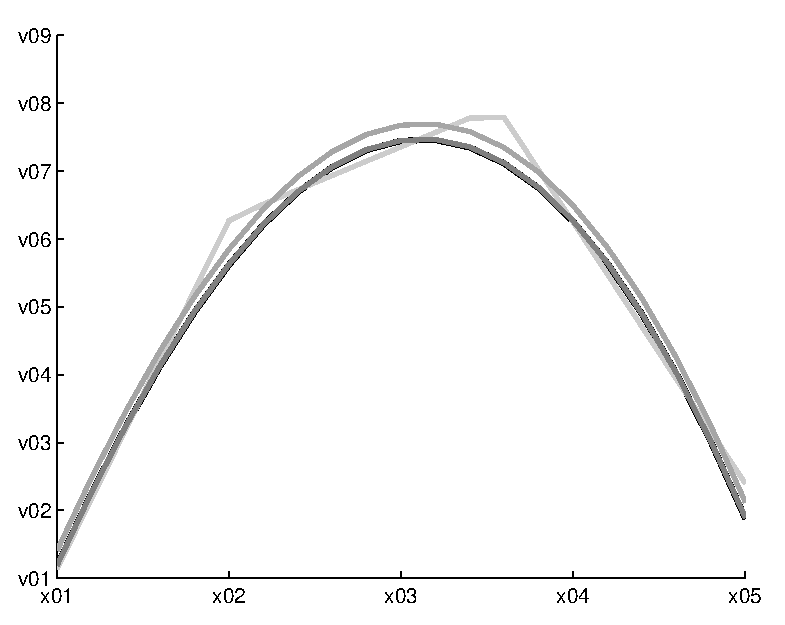
\includegraphics{figures/interior.eps}}%
\end{psfrags}%
%
% End interior.tex
\end{document}
% See http://www.mathworks.de/matlabcentral/fileexchange/loadFile.do?objectId=4638
% for recent versions of laprint.m.
%
% created by:           LaPrint version 3.16 (13.9.2004)
% created on:           15-Feb-2012 20:53:18
% eps bounding box:     15 cm x 11.25 cm
% comment:              
%
\begin{psfrags}%
\psfragscanon%
%
% xticklabels:
\psfrag{x01}[t][t]{0.15}%
\psfrag{x02}[t][t]{0.155}%
\psfrag{x03}[t][t]{0.16}%
\psfrag{x04}[t][t]{0.165}%
\psfrag{x05}[t][t]{0.17}%
%
% yticklabels:
\psfrag{v01}[r][r]{1.42}%
\psfrag{v02}[r][r]{1.44}%
\psfrag{v03}[r][r]{1.46}%
\psfrag{v04}[r][r]{1.48}%
\psfrag{v05}[r][r]{1.5}%
\psfrag{v06}[r][r]{1.52}%
\psfrag{v07}[r][r]{1.54}%
\psfrag{v08}[r][r]{1.56}%
\psfrag{v09}[r][r]{1.58}%
%
% Figure:
\resizebox{0.5\columnwidth}{!}{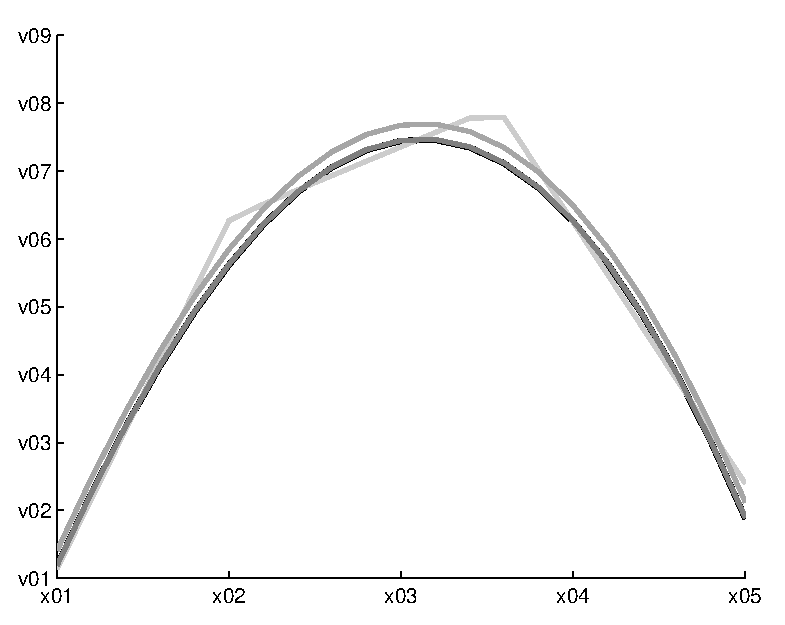
\includegraphics{figures/interior.eps}}%
\end{psfrags}%
%
% End interior.tex
\end{document}
% See http://www.mathworks.de/matlabcentral/fileexchange/loadFile.do?objectId=4638
% for recent versions of laprint.m.
%
% created by:           LaPrint version 3.16 (13.9.2004)
% created on:           15-Feb-2012 20:53:18
% eps bounding box:     15 cm x 11.25 cm
% comment:              
%
\begin{psfrags}%
\psfragscanon%
%
% xticklabels:
\psfrag{x01}[t][t]{0.15}%
\psfrag{x02}[t][t]{0.155}%
\psfrag{x03}[t][t]{0.16}%
\psfrag{x04}[t][t]{0.165}%
\psfrag{x05}[t][t]{0.17}%
%
% yticklabels:
\psfrag{v01}[r][r]{1.42}%
\psfrag{v02}[r][r]{1.44}%
\psfrag{v03}[r][r]{1.46}%
\psfrag{v04}[r][r]{1.48}%
\psfrag{v05}[r][r]{1.5}%
\psfrag{v06}[r][r]{1.52}%
\psfrag{v07}[r][r]{1.54}%
\psfrag{v08}[r][r]{1.56}%
\psfrag{v09}[r][r]{1.58}%
%
% Figure:
\resizebox{0.5\columnwidth}{!}{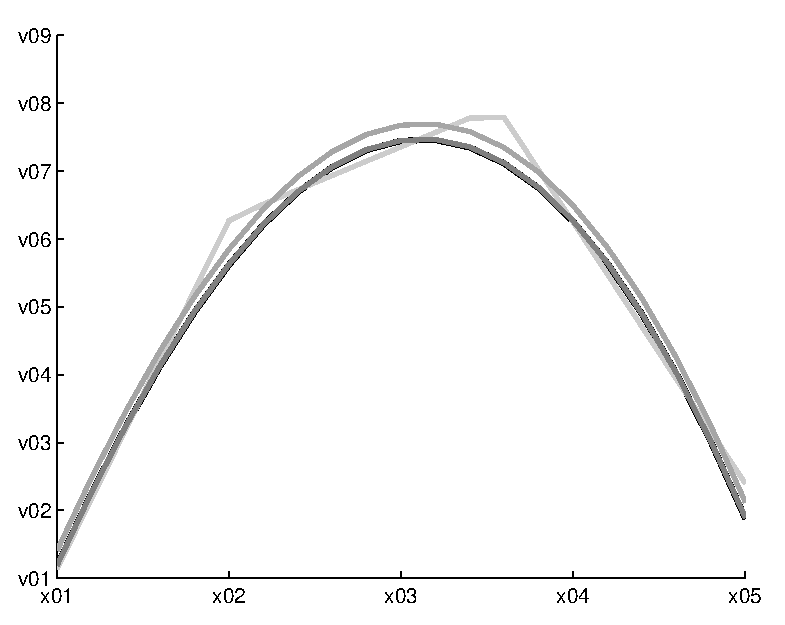
\includegraphics{figures/interior.eps}}%
\end{psfrags}%
%
% End interior.tex
\end{document}
% See http://www.mathworks.de/matlabcentral/fileexchange/loadFile.do?objectId=4638
% for recent versions of laprint.m.
%
% created by:           LaPrint version 3.16 (13.9.2004)
% created on:           15-Feb-2012 20:53:18
% eps bounding box:     15 cm x 11.25 cm
% comment:              
%
\begin{psfrags}%
\psfragscanon%
%
% xticklabels:
\psfrag{x01}[t][t]{0.15}%
\psfrag{x02}[t][t]{0.155}%
\psfrag{x03}[t][t]{0.16}%
\psfrag{x04}[t][t]{0.165}%
\psfrag{x05}[t][t]{0.17}%
%
% yticklabels:
\psfrag{v01}[r][r]{1.42}%
\psfrag{v02}[r][r]{1.44}%
\psfrag{v03}[r][r]{1.46}%
\psfrag{v04}[r][r]{1.48}%
\psfrag{v05}[r][r]{1.5}%
\psfrag{v06}[r][r]{1.52}%
\psfrag{v07}[r][r]{1.54}%
\psfrag{v08}[r][r]{1.56}%
\psfrag{v09}[r][r]{1.58}%
%
% Figure:
\resizebox{0.5\columnwidth}{!}{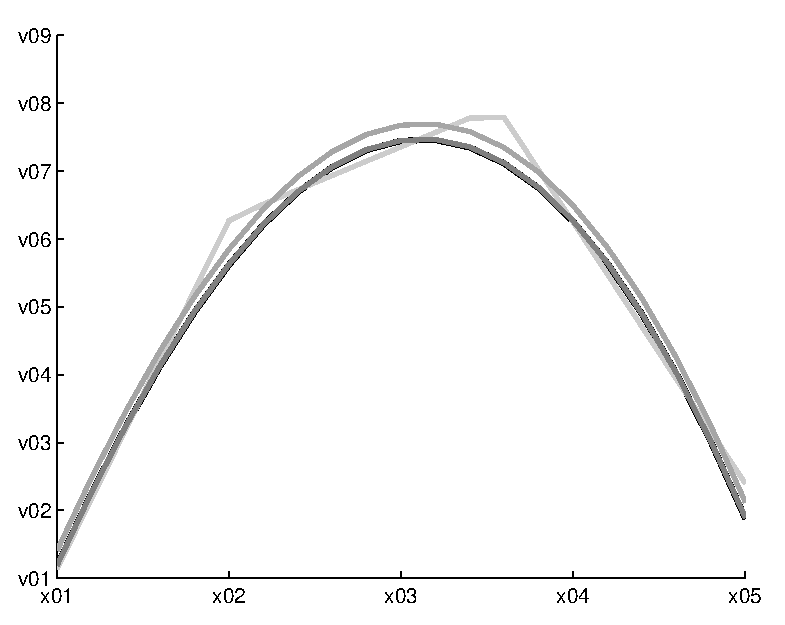
\includegraphics{figures/interior.eps}}%
\end{psfrags}%
%
% End interior.tex
